\documentclass [12pt]{article}
\usepackage{fancyhdr}
\usepackage[utf8]{inputenc}
%\usepackage[english]{babel}
\usepackage{gensymb}
\usepackage{textgreek}
\usepackage{amsmath,amssymb,amsfonts}
\usepackage{algorithmic}
\usepackage{graphicx}
\usepackage{textcomp}
\usepackage[table]{xcolor}
\usepackage{siunitx}
\usepackage{indentfirst}
\usepackage[margin=2.5cm]{geometry}
\usepackage{float}
\usepackage{hyperref}
\usepackage[UKenglish]{datetime}
\usepackage{setspace}
\usepackage{hhline}
\usepackage{amssymb}
\usepackage{lastpage}
\usepackage[acronym]{glossaries}
\usepackage{listings}
\usepackage{color}
\usepackage{booktabs}% http://ctan.org/pkg/booktabs
\newcommand{\tabitem}{~~\llap{\textbullet}~~}
\usepackage{subfigure}
\usepackage[T1]{fontenc}
\usepackage[numbers]{natbib}
\usepackage{helvet}
\usepackage{setspace}
\renewcommand{\familydefault}{\sfdefault}

\definecolor{customgreen}{rgb}{0,0.6,0}
\definecolor{customgray}{rgb}{0.5,0.5,0.5}
\definecolor{custommauve}{rgb}{0.6,0,0.8}

\makeglossaries
\loadglsentries{glossary.tex}

\graphicspath{{images/}}

\hypersetup
{
    colorlinks=true,
    linkcolor=black,
    urlcolor=blue,
    citecolor=black,
}

\doublespacing

\title{}
\author{}
\date{\today}

\begin{document}

\begin{titlepage}
    \begin{center}
        \vspace*{1cm}

        \vspace*{\baselineskip}

        \rule{\textwidth}{1.6pt}\vspace*{-\baselineskip}\vspace*{2pt}
        \rule{\textwidth}{0.4pt}\\

        {\LARGE EXAMPLE TEXT}\\[0.2\baselineskip]

        \rule{\textwidth}{0.4pt}\vspace*{-\baselineskip}\vspace{3.2pt}
        \rule{\textwidth}{1.6pt}\\[\baselineskip]
        \scshape

        \textbf{Student No: 10618407}

        \today

        \vfill

        \vspace{0.8cm}

        
\includegraphics[width=0.4\textwidth]{UOP_Logo.png}

    \end{center}
\end{titlepage}

\newpage
\fancyfoot[R]{Page \thepage \hspace{1pt} of \pageref{LastPage}}
\pagenumbering{roman}
\tableofcontents
\listoffigures
\listoftables
\printglossaries


\setstretch{1.5}

\newpage
\begin{abstract}

    The HEVCS is a project aims to address the challenge posed by the UK Government's ban on the sale of new petrol and diesel cars by 2030 along with the lack of critical charging infrastructure for electric vehicles in the country. To tackle this challenge, the HEVCS has been developed.

    The HEVCS is a more affordable solution than installing a built-in charging circuit and provides a practical alternative for households without access to off-road parking or garages. The HEVCS is charged within the user's home and comes with a vertical dock for easy charging. The user charges the HEVCS platform in their home at their convenience using the provided dock. The user then drives the HEVCS from their house to their vehicle Once they are at their vehicle they drive it underneath, plug it in and begin to charge their car. When the car is charged the user returns the HEVCS to their house and re-docks it.

    The HEVCS has a compact and versatile design with a height of just 110mm, making it suitable for use with most electric vehicles. It features an adjustable payload compartment that can store a battery capacity suitable for the customer’s needs. The batteries used within the payload compartment are recycled batteries that are no longer ‘fit-for-purpose’ from old electric vehicle battery packs. Additionally, the HEVCS can climb kerbs up to 150mm tall, making it suitable for use in both urban and rural environments.

    The HEVCS uses mecanum wheels, which provide advanced control and manoeuvrability that allows the platform to move in any direction, making it an ideal choice for tight spaces.
    Moreover, the HEVCS conforms to class 2 mobility scooter legislation, which means it is considered a pavement vehicle with a maximum speed of 4mph. It achieves this using a tethered controller to allow secure control over the platform's movements. This feature ensures that the HEVCS aligns with the safety regulations for class 2 vehicles.

    In summary, the HEVCS is a practical choice of vehicle charging solution which incorporates a compact design, adjustable payload compartment, mecanum wheels, and an affordable price. The HEVCS offers a viable alternative to the current lack of charging infrastructure in the country, providing an accessible way for individuals to transition to electric vehicles.


\end{abstract}
\section{Acknowledgements}

The team would like to express our gratitude to the following individuals and organizations both internal and external to the university for their invaluable contributions to this project:

Firstly, we would like to thank James and Heather Sirmon from Sirmon Industries ltd. for providing the initial specification for the project as well as for covering a large amount of the project’s costs. We would also like to thank Jake Gibson Shaw-Sutton for being the external supervisor for this project along with Jo Byrne and the European Social Fund for organising and facilitating this project.

We extend our appreciation to Dr Paul Davey for being our project module leader and providing us with additional ideas to enhance our project. We are also thankful to Dr Hazel Sales for her insights into English grammar and writing for engineering, which significantly improved the clarity of our report. We also acknowledge the assistance of Dr Alan Malvern for providing us with ideas for and marking our patent landscape document, and Martin Simpson for allowing us to access SMB 209 for use as our laboratory and for general help in the labs. We extend our appreciation to Anna Hansen and Doyel Sengupta for sorting out all the component orders and ensuring timely delivery of materials, without which this project would not have been possible.

We further our appreciation to Rick Preston for his assistance in cutting the aluminium extrusion facilitating the use of the university’s Workshops. We are also grateful to Dave Pattison from W6 for undertaking the metal work for this project.

Finally, we would like to express our gratitude to the campus coffee shops for providing us with warm cups of coffee and cake to get through the long days, and the support staff for helping us with general queries surrounding procedure and laboratory assistance throughout the project.

The team would also like to thank their family and friends for their continued support and inspiration through this project and university.


\newpage
\pagenumbering{arabic}
\section{Introduction}
\setcounter{page}{1}

In recent years, the automotive industry has experienced a surge in the sales and adoption of electric vehicles (EVs). This increasing market demand for EVs reflects a growing consumer preference for sustainable transportation solutions that reduce carbon emissions and dependence on fossil fuels. However, despite the rapid growth in EV sales, the implementation of charging infrastructure has not kept pace with the exponential expansion. This discrepancy between the increasing number of EVs on the road and the limited availability of charging stations has emerged as a critical challenge, impacting the overall convenience and acceptance of electric vehicles.
However, the slow pace of charging infrastructure development poses a significant hurdle to the widespread adoption of EVs. The availability of public charging stations is limited, particularly in regions or areas with inadequate infrastructure planning. This situation creates challenges for EV owners, as they face concerns regarding range anxiety and the availability of convenient and accessible charging options. The imbalances between EV adoption and the charging infrastructure rollout not only affects individual EV owners but also impacts the overall perception of EVs among potential buyers, influencing their decision-making process.
The continued growth and adoption of EVs requires a concerted focus on addressing the disparity between charging infrastructure and EV sales. The Home Electric Vehicle Charging System (HEVCS) has been developed to bridge this gap. By offering a portable charging solution, the HEVCS enables EV owners to conveniently charge their vehicle without relying solely on fixed charging infrastructure. The HEVCS caters to diverse user demographics, ensuring accessibility and usability for individuals of all abilities.
The primary objective of the HEVCS is to provide flexibility to users by being driven directly to the EV, eliminating the need for fixed charging points in residential areas. With the HEVCS ability to navigate kerbs, it ensures the ease of operation for individuals with varying levels of mobility or strength.
This report discusses current technologies trying to improve the charging infrastructure and identifies the gap that the HEVCS is trying to fill. It also discusses the design architecture and evaluate the operation of the HEVCS. Moreover, it will explore the potential benefits and implications of integrating the HEVCS into the existing EV market, considering factors such as user experience, charging efficiency, and environmental sustainability.
The development of the HEVCS addresses the gap between EV sales and charging infrastructure, offering a portable solution for EV owners. By examining the technical aspects, operational features, and potential impacts of the HEVCS, this report aims to aid in the understanding of the charging platform and its role in shaping the future of electric vehicle adoption.


\newpage
\section{Literature Review and Prior Art}
The increasing prevalence of electric vehicles, especially as a response to numerous governments’ impending bans on petrol and diesel vehicles, has led to a breadth of research and developments around charging infrastructure. 

EVAR is one company creating robotic solutions to charging electric vehicles. One of their flagship products, Parky, is an EV charging robot\cite{EVAR_PARKY}. However, Parky is specifically designed for use within multi-storey carparks, and not within domestic environments. One of Parky’s benefits is the fact that only sockets must be fitted around the car park, the power circuity is provided within the robot. Once a car is parked and plugged in, a Parky instance is summoned to the parking space, plugging itself in and providing power to the socket. Parky uses a combination of LiDAR, Ultrasonics, and bump sensors to guide itself, with a QR code used to recognise the connector.

Another EVAR product is their Mobile EV Charger, a motor driven shopping-trolley sized cart containing EV batteries\cite{EVAR_MOBILE_CHARGER}. The device is charged at a wall charger, before being driven to where the EV is parked. It uses Muscular Strength Enhancement technology as the human-robot interface, directly correlating motion on the push-bar with drive system inputs, making the product “as easy to use as a shopping cart”. As with their other products, a combination of ultrasounds and LiDAR is used to prevent the cart being driven into obstacles. 

One disadvantage of both these products is their design assumes a perfectly flat driving surface, such as in a multistorey carpark. This cannot be guaranteed in public spaces such as pavements. Furthermore, neither product contains provisions for traversing kerbs, something that would be necessary for street use. The 750kg weight of the EVAR mobile charger would require several people to move up or down a kerb. A common parking layout on UK roads is having cars parked along one or both sides of the road, leaving only room for a single line of traffic to pass through. Neither product would be useful in such an environment; space is a premium of which none can be spared.

Electric Car Manufacturer NIO offer a “Mobile Charging Service”, where upon user request, a van with car charging equipment is dispatched\cite{nio-power}. Providing approximately 100km of range in 10 minutes, the system is designed for infrequent use, as a range extender or in cases of lack of charger availability. For its intended purpose of plugging gaps in charging infrastructure, it is suitable. However, such a system would be completely inadequate for widespread use as a replacement for public charging systems.

NIO has also installed rapid battery swapping stations throughout its service areas\cite{nio-power}. Capable of swapping a compatible EV’s batteries in three minutes and performing automated battery health checks. Whilst fast, these battery swapping stations have limited compatibility, and standardisation amongst manufacturers would be needed to prevent fragmentation of services between different manufacturers. Furthermore, such stations are large and expensive to fit, limited how they could be deployed.

Behl et al.’s work describes using a TurtleBot 3 Waffle-Pi as the basis for an electric car charging robot\cite{behl2019autonomous}. However, the TurtleBot only acts as a proof-of-concept for car park navigation, and the team did not attempt to integrate the additional functions of battery swapping and armature-based autonomous plug connection. The Waffle-Pi is only 141mm tall, however lacks the carrying capacity that many of the larger platforms have. Both EV batteries, and the auxiliary equipment needed for charging applications, are heavy. However, as a test platform for navigation and mapping algorithms, the Waffle-Pi is ideal.

Behl et al. also identified the potential of battery swapping technology, such as in NIO’s battery swapping stations, identifying the same issues that the NIO stations fall afoul of\cite{behl2019autonomous}. The work suggested that a vertical design would be an improvement, reducing the required ground space at the cost of additional mechanical complexity. The concerns around standardisation of battery designs were also shared, placing further emphasis on the need for some form of standardisation. Standardisation would have numerous benefits for competition and innovation, further driving development[SHIN2015152].

Walz et al.’s work identified the need of powerful vision and positional systems for fully automated electric vehicle charging\cite{walzel2019robot}. Not only must the connector type be correctly identified, its facing and aspect must also be identified. Failure on either side could lead to damage to both the connector and the robot’s charging equipment. 

Afshar et al.’s review paper into mobile charging technology as a field of research identified the need to keeps costs to a minimum and for public charging solutions to have adequate balancing of supply and demand to reduce grid imbalances\cite{afshar2020literature}. Contrasting with these challenges, the review also further extolled the potential benefits of mobile charging technologies for EV owners and the energy grid. Reduced range anxiety; increased charging availability; lowered risk of grid failure; all potential benefits of widespread mobile charger adoption. Range anxiety continues to be a large barrier to EV adoption, technology that reduces its propagation will only aid in EV adoption[NOEL201996, NEUBAUER201412].

One common trait each of these reviewed products included being unsuitable for filling the domestic charging gap observed in the UK market. Each solution is either over specialised, too costly, too big, or lacks the needed capacity. An alternative approach must be taken, focussing on minimising size and cost, without compromising charging capacity to the point at which it becomes unfit for purpose.

\newpage
\section{Business Justifications}

\subsection{Research Techniques and MECE Analysis}

The team engaged in innovation talks throughout the project, particularly with 42Technology \cite{42T}, to understand the framework commonly used to solve complicated problems within industry. A particular method used involved the definition of the problem broken down into mutually exclusive sub-problems that are collectively exhaustive. This method is referred to as \gls{mece} Analysis and enabled the team to focus on various elements of the project to achieve one shared goal, without overlapping or reproducing any work.

This method aided the understanding project criteria from the sponsor’s perspective regarding patenting, and from the university’s perspective of academic evaluation. The PEP defined the market gap, drawing from research gathered that detailed the lack of EV charging infrastructure within the UK, and how realistically, the public cannot rely on shared charging points. However, \gls{mece} analysis has uncovered the \gls{hevcs} as a feasible solution to such a challenge, and that the situation would benefit from having a mobile, versatile approach to suit the varied requirements of \gls{ev} users in different locations around the UK.

\subsection{Addressing the Key Challenges of Electric Vehicle Adoption}

The common barriers preventing the public from purchasing EVs being price, range and charging infrastructure. The \gls{hevcs} tackles all three of these problems, and the team have designed the platform and its use specifically for its application within the real-world.

\subsubsection{Charging Infrastructure and Trends in Usage}

Currently, the UK Government’s National Traffic Survey stated that 938,182 electric cars were registered to be on the roads as of Q3, 2022 \cite{Q32022}. Comparatively, a survey published in October 2022 stated that 34,637 public charging points were currently installed \cite{chargestats}. These figures indicate that the charging infrastructure available cannot keep up with the current number of \gls{ev}s on the road and raises concerns as this number is set to rise with the 2030 ban on selling new petrol and diesel vehicles. Furthermore, it is predicated that 99\% of miles will come from \gls{ev}s by 2050, a figure that has been adjusted after an underestimation of their adoption rate \cite{2050rates}.

Approximately 50\% of UK charging points are placed at end of journey destinations, typically within car parks the public frequent for shopping, leisure, and down-time activities \cite{chargestats}. A Government survey revealed a majority's preference to charge \gls{ev}s at home, with 66\% and of \gls{bev} and 41\% of \gls{phev} users had their own dedicated charging point within a private driveway or garage \cite{homecharge}. The survey highlights that users felt dedicated charging points were either too expensive or complex to install.

Conversely, 53\% of the UK do not have a driveway or garage that would allow for the possibility of installing a domestic charging point. This has proven to be a deciding factor in the public adoption of \gls{ev}s. The portion of the market purchasing \gls{bev}s \ \gls{phev}s using public dedicated charging points within the vicinity of their residence is 4\% and 1\% respectively \cite{chargestats}. Thusly, a market gap to provide a product that can charge EVs within the immediate surroundings of the home has been identified. Moreover, the \gls{hevcs} does not require a dedicated parking space, and can be used at the individual's discretion.

\subsubsection{National Grid Demands}

When considering the typical commuting patterns, full-time workers with typical 9-5 jobs are amongst those susceptible to aligning their arrival to domesticated regions. 60\% of EV users prefer to charge between 5-8pm, meaning the national grid struggles with the demand of those coming home, with up to 20\% of the UK's EV fleet charging between those hours \cite{chargestats}. The \gls{hevcs} could charge during the off-peak times, lessening the load on the grid.

\subsubsection{Battery Range and Efficiency}

The National Travel Survey presented statistics in 2021 stating that 98.5\% of journeys taken in the UK were less than 50 miles \cite{nts}. The capacity of the payload compartment was calculated through an analysis of both power consumption and efficiency, conducted using data from the UK public’s current \gls{ev} usage trends. The average efficiency determines that 1 kWh equates to approximately 3.5 miles, and second-hand EV batteries typically have a capacity of 80-90\% of the original value \cite{strickland2014estimation}. The \gls{hevcs}’s configurable payload compartment can supply the user with 10 to 50 miles of range, depending on the \gls{ev} batteries used, as shown in the research and calculations section.

\subsubsection{The Cost of Charging an Electric Vehicle}
The \gls{hevcs} presents itself as a cost-effective product that reduces the price of charging an \gls{ev}. Within the UK, domestic electricity prices have been on the rise, and the cost of charging at public points has increased. Furthermore, the spaces in which to charge are not guaranteed, a free to park still must be paid. A cost analysis presents the additional benefits of an individual having their own \gls{ev} charging device, such as the \gls{hevcs}, that remains domestically powered.

Providers, such as EDF Energy \cite{edf}, offer \gls{ev} charging tariff that allow the user to charge their vehicle for 9p per kWh during off-peak times, oppose to 46p per kWh at public charging points within Plymouth. The typical UK driver makes 14 trips a week, each with an average distance of 8.4 miles, equating to an annual mileage of $ \approx 6,000 $ miles. This results in a running cost of £788 for vehicles with an efficiency of $ \approx 3.5 $ charging on public tariffs. By using the reduced domestic tariff, the user would spend £154 a year, the savings of which would accumulate to cover the price of the \gls{hevcs} platform over a span of several years.

\subsubsection{Environmental Benefits}
The \gls{hevcs} can give a second life to \gls{ev} batteries, while educating users on the importance of understanding their daily commute, and what it demands in terms of power. In addition, it is understood that frequently charging \gls{ev} batteries to their maximum capacity, and letting them discharge fully, reduces their lifespan \cite{haram2021feasibility}. This device can bridge the learning gap, educating users on what it means to operate a battery within its ideal state of charge range to improve longevity.
It is common knowledge that EV batteries are designed to possess an ability to retain their original battery capacity over many years, but its ability to do so depends on a variety of factors. Charging schedules that keep the state of charge between 20-80\% would provide an adequate amount of power to fulfil the average daily commute. Moreover, the \gls{hevcs} would allow the user to take advantage of off-peak electricity rates, smart charging features, and monitoring energy consumption. Through adopting a maintenance charge approach, following the natural patterns to meet the user’s everyday needs, the user can identify how to adjust their habits to positively impact batter health and costs.


\newpage
\section{Requirements}\label{sec:req}

\subsection{Dimensions}

To determine the compatibility of the \gls{hevcs} with existing \gls{ev}, a comprehensive survey was conducted on a sample of 40 recently released EV models. The survey aimed to evaluate two critical dimensions: ground clearance and distance between tyres. These dimensions play a crucial role in determining whether the \gls{hevcs}platform can be driven underneath the EVs and accommodate their specific characteristics.

Based on the survey results, the average ground clearance of the sampled EVs was determined. By considering the range of ground clearances across the surveyed models, an average value of ground clearance was calculated. This average ground clearance serves as a benchmark for the maximum height of the \gls{hevcs} platform, ensuring that it can safely fit underneath the majority of new EVs entering the market. Notably, the survey findings revealed that the \gls{hevcs} platform, with a maximum height of 155mm, would be compatible with approximately 53\% of the surveyed EVs, enabling seamless integration and operation.

In addition to ground clearance, the distance between tires, or the wheelbase, is a crucial factor to consider when assessing compatibility. Through the survey, the average wheelbase of the sampled \gls{ev}s was determined to be 2584.87mm. This measurement represents the average distance between the front and rear wheels of the surveyed EVs. By accounting for the typical tire diameter of 457.2mm, it is possible to estimate the average distance between the tires, which was found to be approximately 2127.67mm. This information is valuable for designing the \gls{hevcs} platform, as it ensures that the platform can accommodate the average wheelbase of EVs and align its components accordingly.

Considering door clearances is another important aspect when assessing compatibility between the \gls{hevcs} platform and \gls{ev}s. In the context of the UK, door clearances typically range between 762mm and 838mm. By incorporating these door clearance values into the design considerations, the \gls{hevcs} platform is designed to pass through doorways without any issues, allowing for smooth integration with existing infrastructure and ensuring seamless access to buildings or designated areas.

By conducting a meticulous survey of 40 new EV models and analysing key dimensions such as ground clearance, distance between tires, and door clearances, the compatibility of the \gls{hevcs} platform with existing EVs can be assessed in detail. This comprehensive evaluation enables the design team to make informed decisions, ensuring that the \gls{hevcs} platform aligns with the specifications of the majority of EVs in the market, facilitating integration, compatibility, and efficient operation.

\subsection{Structural Integrity}

In light of the platform's maximum height constraint, which should not exceed 155mm, it is imperative to determine the maximum allowable wheel diameter. Based on this constraint, the wheel diameter is established as 150mm. Moreover, in compliance with class 2 mobility legislation, the platform is subject to a speed limitation of 4mph (equivalent to 1.79m/s) and a maximum weight capacity of 113.4kg.

With these parameters at hand, the team calculated the platform's maximum power and torque requirements. Considering the maximum weight condition, where the craft is carrying its full capacity of 113.4kg, each motor must exert a force of 278.11N to counteract gravity. This force is essential for maintaining stability and facilitating the robot's locomotion.

Given the fixed wheel diameter of 150mm and a linear speed of 4mph (1.79m/s), the angular velocity of the wheel was deduced. By employing the formula $ v = \textomega * r $, where v represents linear velocity, \textomega denotes angular velocity, and r signifies the wheel radius, the equation was rearranged to solve the angular velocity. In this case, the angular velocity was calculated to be approximately 23.87 rad/s.

Subsequently, the team determined the torque required to achieve this angular velocity. The equation $T=Fr$, where T represents torque, F denotes the force on each wheel, and r signifies radius of the wheel, was used Assuming constant angular velocity \textomega and negligible frictional losses, the torque required was computed to be approximately 20.86Nm.

Furthermore, we can derive the maximum power output required by the platform. Employing the equation $ P = T* \textomega $, where P represents power, we multiply the torque (T) by the angular velocity \textomega to obtain the maximum power output, which was found to be approximately 497.93W.

In addition to the previously mentioned requirements, the outdoor utilization of the platform necessitates its ability to navigate various challenging situations. These include driving on uneven terrain, overcoming obstacles, adapting to environmental conditions, maintaining stability on slippery surfaces, and traversing inclines.

The terrain outside differs significantly from controlled indoor environments. It can feature irregular surfaces with variations in elevation, such as gravel paths, grassy fields, or rough terrain. Failure to consider these factors in the design can lead to complications for the platform's operation. Therefore, robust design considerations should be made to ensure effective performance on uneven terrain while maintaining stability and preventing damage to the craft.

Moreover, the platform's operation will be subjected to changing environmental conditions throughout the year. It should be capable of withstanding various weather conditions, including rain, snow, high humidity, or extreme temperatures. To address these requirements, the platform should possess a minimum Ingress Protection (IP) rating of IP55, providing adequate protection against water and dust ingress.

In colder climates, surfaces can become icy, posing a significant challenge for the platform's traction and control. To ensure smooth and safe operation, the platform should be equipped with suitable mechanisms or materials that provide optimal grip and prevent slipping on icy surfaces.

Furthermore, outdoor paths may not always be flat, necessitating the platform's capability to traverse inclines. As per the class 2 mobility scooter legislation, the platform should be capable of coming to a stop on a slope of 1 in 5, which requires appropriate power, control, and braking mechanisms to ensure safe operation and prevent unintended rollbacks.

\subsection{Kerb Climbing}

A prominent capability of the platform is its ability to negotiate kerbs, providing users with the convenience of effortless transportation to their vehicles without requiring physical exertion. Considering the platform's maximum weight capacity of 113kg, it is crucial to ensure that it can smoothly ascend and descend kerbs without causing instability or damage. To establish a target for the kerb height that the platform should be able to traverse, a comprehensive survey of kerb heights in the local area was conducted.

During the survey, a representative sample of kerbs was assessed to determine the average height encountered. By considering various locations and situations, such as residential areas, commercial districts, and public spaces, the survey aimed to capture the diverse range of kerb heights that the platform is likely to encounter in real-world scenarios. Upon careful analysis, the average kerb height was found to be approximately 150mm.

Setting the target kerb height at 150mm provided a benchmark for the platform's design and performance. It ensured that the platform could accommodate the typical kerb heights encountered during everyday use, allowing users to seamlessly navigate kerbs without requiring additional effort or assistance. Incorporating appropriate mechanisms, such as robust suspension systems, efficient power delivery, and suitable wheel designs, will facilitate the smooth traversal of kerbs and enhance the platform's overall usability.

\subsection{Safety Features}

To ensure the safe and effective use of the \gls{hevcs}, several critical safety considerations must be taken into account. Given that the platform is intended for use by any member of the public, incorporating collision avoidance features becomes paramount to enhance ease of use and prevent potential accidents.

In addition to collision avoidance, it is essential to provide users with assistance regarding the capabilities and limitations of the platform. This information empowers users to make informed decisions and operate the platform safely. For instance, the system can provide feedback to the user regarding the platform's ability to navigate specific obstacles or terrains. This includes informing the user whether the platform can safely climb a given kerb height or assessing the steepness of a slope to determine if it exceeds the platform's capabilities. By offering this assistance, users can avoid situations that may pose a risk to their safety or the proper functioning of the platform.

According to Class 2 mobility scooter legislation, it is specified that the craft cannot be controlled remotely. Consequently, the controller for the platform will need to be tethered, ensuring that the operator maintains physical contact and direct control over the vehicle. This requirement ensures a higher level of safety and control, as it eliminates the potential risks associated with remote control operation. Furthermore, to address potential situations where the connection between the controller and the platform is lost, a fail-safe mechanism must be implemented. In such cases, the platform should be designed to immediately stop its movement to prevent unintended and uncontrolled motion, thereby prioritizing user safety and preventing the craft from rolling freely, potentially causing accidents or damage.

Implementing these safety features requires a comprehensive integration of sensor systems, advanced algorithms, and user interfaces. It is crucial to employ reliable and accurate sensors to ensure precise detection and assessment of the environment. Furthermore, developing robust algorithms capable of real-time analysis and decision-making is essential for timely collision avoidance and accurate user assistance.


\newpage
\section{Optioneering}

\subsection{Hardware Justifications}

\subsubsection{Microcontroller Selection and IDE}
STM32 boards were chosen as they provide scalability in terms of hardware resources and software development tools through the use of mbed. With a wide range of microcontroller options available, the team were able to choose the STM32 board that best suits the project requirements, such as processing power, memory capacity, and peripheral integration. This scalability enables the testing of software on different STM32 platforms, ensuring compatibility and performance across all three platforms.

STM32 boards are known for their robustness and reliability. The microcontrollers are designed with built-in features that enhance the reliability of software, such as memory protection units, error correction codes, and fault detection mechanisms. These features contributed to the stable and dependable operation of the platform, reducing the likelihood of software failures and improving overall system reliability. Furthermore, the STM32 boards used are  compatible with various \gls{rtos}, providing scheduling and multitasking capabilities. This allowed the team to test and evaluate the software's behaviour under real-time constraints. This enables the validation of time-critical functionalities, responsiveness, and task management, ensuring reliable and deterministic system operation. Finally, the boards offer excellent integration capabilities with external testing equipment and tools, such as debuggers and pico-scopes. This integration enables comprehensive hardware and software debugging, performance monitoring, and analysis, facilitating in-depth testing and troubleshooting.

\subsubsection{F429ZI}
This section provides an analytical comparison of the STM32F429ZI microcontroller against alternative options for embedded systems requiring reliability, multithreading capabilities, and diverse communication interfaces. It investigates the suitability of the STM32F429ZI microcontroller for interfacing with switches, joysticks, \gls{vesc}s, and servos. By considering its technical specifications, architectural features, and development ecosystem, the decision to use this board was backed up by its various abilities.

Embedded systems play a crucial role in modern technological applications, encompassing a wide range of industries such as robotics, automotive, and industrial automation. The selection of an appropriate microcontroller for a given application is paramount to ensure reliability, efficient multitasking, and seamless communication with external devices. In this regard, the STM32F429ZI microcontroller presents a compelling option due to its exceptional features and capabilities. It is built upon the high-performance ARM Cortex-M4 core. Its rich set of peripherals and advanced architecture make it a prime choice for complex embedded systems. Noteworthy specifications include a clock speed of up to 180 MHz, ample flash memory and \gls{ram}, and a versatile set of communication interfaces, such as \gls{uart}, \gls{spi}, I2C, and USB.

Multithreading is a critical aspect of this project as it requires efficient execution of concurrent tasks. The STM32F429ZI microcontroller supports multithreading through its advanced interrupt handling mechanism and hardware-based multithreading support. This feature allows for the seamless execution of multiple tasks simultaneously, enhancing overall system performance and responsiveness. Furthermore, reliability is a key requirement in mission-critical applications. The STM32F429ZI microcontroller excels in this aspect by incorporating error correction codes (ECC) in its memory system, ensuring data integrity and fault tolerance. Additionally, its robust power management features, low-power modes, and built-in watchdog timers contribute to the overall system's reliability and fault resilience.

The ability to communicate with various external devices is an essential requirement of this project. The STM32F429ZI board offers a multitude of communication interfaces, allowing seamless integration with controller peripherals, as well as the \gls{vesc}s and servos. The flexibility regarding \gls{gpio} pins, \gls{pwm} outputs, and dedicated hardware interfaces provide the necessary capabilities to interface with these devices efficiently. The use of \gls{api}s for which are detailed in the official STM32 documentation. These include reference manuals, datasheets, and application notes, providing valuable information on hardware features, software development guidelines, and testing methodologies. The platform offers an extensive collection of pre-built libraries, encompassing diverse functionalities such as communication protocols, sensor interfaces, motor control, and more. Leveraging these libraries not only saves significant development time but also facilitates the rapid prototyping of complex projects, such as the \gls{hevcs}. Consequently, pairing these factors with the team’s familiarity with ARM Cortex-M based microcontrollers, development with the STM32F429ZI was intuitive in nature and accelerated the embedded system’s functionality.

\subsubsection{L432KC}
The \gls{hevcs} controller required a compact microcontroller to integrate an \gls{lcd} display, D-pad buttons, and \gls{spi} communication. The STM32L432KC controller’s technical specifications, architectural attributes, and performance advantages met the requirements of the targeted features. Furthermore, the board is recognised for its low power consumption, operation efficiency, and its use within portable applications. The \gls{lcd} operates using hardware accelerated graphical features, such as DMA-driven memory transfers. The \gls{gpio} pins have multiple configurations and include external interrupt controllers facilitate the D-pad input processing. The STM32L432KC includes multiple \gls{spi} peripherals that enable high-speed data transfers over the \gls{spi} bus, minimising CPU overhead.

The STM32L432KC microcontroller outperforms most Arduino boards in terms of processing power, thanks to its advanced ARM Cortex-M4 core. The STM32L432KC's high clock speed enable efficient execution of complex algorithms, making it suitable for applications that demand real-time processing, data manipulation, and signal analysis. Unlike Arduino, the STM32 family allows developers to delve into low-level programming, giving them greater control over hardware resources. The microcontroller supports the C/C++ programming language, and developers can directly access registers and peripherals, optimizing performance and resource utilization. The team believe this level of customizability is particularly beneficial for this project, following from research into applications that require fine-grained control over system behaviour.

\subsubsection{ESP-8266}
Within this project, the ESP-8266 presents itself as a low-budget option capable of reliable data saving capabilities using Wi-Fi. It has a compact design with a vast range of peripherals available. Its highly integrated System-on-a-Chip (SoC) architecture reduces requirements for additional components. Its enhanced power management features enable the ESP to be used during periods of long-term operation on a limited power source. Through examination of the features, its network connectivity was enhanced within the project. The ESP-8266’s ability to connect to the internet using Wi-Fi opens a plethora of opportunities for \gls{iot} applications. The support provided includes various options regarding networking protocols, with detailed guides on how to implement each.

\subsubsection{Pi Pico}
The Raspberry Pi Pico was chosen to manage the LiDAR sensors for a variety of reasons, all of which made them more suitable than competing boards. The cheap cost and small size, at less than £4 each and measuring 20x50mm, allowed them to easily be mounted around the chassis, without taking up space better suited for the battery payload or other control systems.
In sensing applications, especially ones as safety critical as monitoring the LiDARs, minimised latency is key. The Pi Pico uses a UK-designed RP2040 microcontroller, featuring an Arm Cortex-M0+ processor, with dual cores running at a maximum of 133MHz. This dual-core architecture allows for true multitasking, as opposed to the 'multithreading' implementations seen using the MBED RTOS on the F429zi, where clever use of the scheduler mimics the ability to multitask. This functionality proved ideal for multiple purposes, with communication between boards often delegated to one of the cores, allowing the second core to solely manage sensor reading and data processing.
Whilst the 133 Mhz clock speed of the M0+ is beaten by the maximum 180MHz capable of the Cortex M4, the dual core capability effectively doubles the number of instructions performed per second, providing unparalleled flexibility for the price point. The 264Kb of SRAM matches that of the F429ZI, and whilst more RAM is undoubtably a positive, this amount proved adequate for the purpose, especially when needing to compensate for MicroPython's more laissez-faire approach to memory management.
Pimoroni, who manufactured the chosen breakout boards for the VL53L5CX, supplied firmware written specially for the Pi Pico in MicroPython. This, combined with a prior familiarity with MicroPython, alongside unreliable support for the C SDK, further pushed towards the Pi Pico over an STM32-based microcontroller board.
With just ~91mA of power consumption in a wake-state, the Pi Pico draws a miniscule amount of power, especially in comparison to the drive systems and other ancillary parts of the HEVCS system. However, power efficiency should always be taken into consideration when designing a system. By minimising power use by the MCUs, more power can be allotted for the drive systems, increasing range.


\subsubsection{Super500 Servos}

e Super500 applications suit that of the project, with a high level of accuracy and sufficient holding force. The servos are used to adjust the angle of the motor mounts to orientate and lift a platform weighing a maximum of 113.4kg up and down kerbs 150mm in height, providing the force defined in the requirements. As solenoids were used to hold the arms in a rigid, flat position, the servos only consumed power when articulating the arms, making the robot much more efficient when carrying the payload.

A single servo was used in each arm to lift the robot by 30 degrees. The servos used 0.4A each, meaning that lifting the whole platform with additional weight equating to roughly 40kg consumed 1.6A. However, the final design used two motors on each side of the robot, ensuring that a full weight of 113.4kg could be lifted.  Rounding up the supply current to 2A per hour, with a battery voltage of 24V, with 90\% efficiency, the robot can rotate between articulating its arms and holding the position for 90 minutes using 3000mAh li-po batteries. The configuration of the robot currently uses one battery per servo, however, considering the run-time of the articulation methods, and the lower supply current, these servos could use power from the same source. Altogether, the four servos would require 19.2wh from the main battery, a result the team believes to be efficiently optimised.

\subsubsection{6384 Motors}

The team established that the 6384 motor was used in a lot of hobbyist projects that had similar applications as the \gls{hevcs}. These motors have a high-power output, making them suitable for applications that need a lot of torque. Similar projects include electric skateboards, bikes, and drones. Brushless motors have a longer lifespan and require less maintenance. Furthermore, less noise and vibration allows for smoother operation of the platform.

The motors are highly efficient compared to brushed motors due to having fewer parts and less friction. This results in more energy being converted into mechanical energy, and less energy lost in the form of heat. Brushless DC motors are capable of handling more precise speed control, an essential aspect of this product as it will operate around people.

Upon reflection, the team feel that the 6384 motors and Super500 servos were appropriate choice for the project due to their ‘plug-and-play’ usability. Furthermore, the \gls{bldc}s were easy to configure when paired with the speed controller. Their size meant that they aligned well with the extrusion, incorporated into a compact motor drive compartment. Additionally, later improvements to the \gls{hevcs}'s design meant that the motors and necessary driver equipment were contained in modular units. This means that they were all identical, easy to install, and maintain. Furthermore, if the \gls{hevcs} were to break when in use by a customer, new units could be installed with ease.

\subsubsection{LiDAR Selection}

Light Detection and Ranging (LiDAR) sensors typically come in one of two types, mechanical and solid-state. Mechanical LiDARs use mechanical components to rotate the LiDAR sensor through 360°, taking thousands of samples per second. Solid-state LiDARs are typically a single sensor on a chip, fixed in position. Mechanical LiDARs are a mature technology, well established within industry applications, however are bulky and extremely expensive. The SLAMTEC RPLIDAR S2M1-L18 costs £299.99, and the LEISHEN AGV Anti-Collision LiDAR increases that to £656.25 \cite{robotshoplidar}.
An additional downside of mechanical LiDARs, and the vast amount of high-resolution point-cloud data they produce, is the data must be processed in some way. Many robots use the Robot Operating System’s sensor interface framework, with its publisher-subscriber model, to help process the data, alongside software running on an on-board desktop CPU running a Linux instance. This would be unfeasible given the selected MCUs, and the size and power requirements of the robot.
Solid state LiDARs, such as the chosen VL53L5CX are significantly more compact, measuring at just 19x19x4.6mm. They also cost significantly less, at £19.50 including the breakout board. With a viewing angle of 63° diagonally and 44.5° horizontally, they wide coverage for their price point. With 64 samples at a maximum of 60Hz, the VL53L5CX generates 3,840 samples per second, enough for high accuracy detection of obstacles at up to four metres. Single Photon Avalanche Diodes act as the receiver array, providing high sensitivity to even single-photon responses. Built-in histogram analysis automatically removes cross-talk induced by protective glass covers, allowing for the sensor to be fully enclosed without affecting its accuracy. No sensor on the market matched the VL53L5CX for performance at it’s price point, and its main weakness, the limited field of view, could easily be solved by positioning multiple around the design. Even after purchasing eight, it is still around half the cost of the SLAMTEC S2L1-M18, and resulted in 30,720 samples per second, near-parity with the S2L1-M18’s 32,000 samples per second \cite{robotshopanticol}.

\subsubsection{IMU Selection}
The MPU6050 by InvenSense was chosen as the IMU of choice. Combining a 3-axis gyroscope and accelerometer onto the same chip, alongside onboard motion processing to extract information from the readings taken. Capable of measuring values of up to 2,000°/s, and up to +/- 16Gs, the MPU6050’s upper and lower limits far exceed any movement the platform will be capable of undertaking. Additionally, each MPU6050 only draws 11mW of power, ideal for MCU applications.
Available as a breakout board for less than £5, and using an I2C interface, the MPU6050 was ideal for our requirements of a low latency inertial measurement unit. Comparable units, such as the MPU6000, or the more powerful MPU-6500 were considered. The MPU6000 is functionality identical from a sensor’s perspective, only adding an SPI interface. As I2C had already been chosen as the interconnect medium, this provided little benefit. In contrast, the MPU6500 is significantly more powerful, providing 32KHz gyro updates while consuming only 6.1mW. However, this comes at the cost of drastically increased vibration sensitivity, leading to soft mounting being almost mandatory. Given the low speeds and resolution required of the IMU, the 6500 would greatly exceed the necessary specification, and costing £7.63 for just the chip, are much more expensive than the 6050.

\subsubsection{Multiplexer Selection}
The SN74LV4052A Dual 4-channel multiplexer was chosen to allow a single UART peripheral to control all four sensor boards \cite{SN74LV4052A}. Dual input/output with 4 channels made it well suited for UART’s two-line tx/rx protocol, and four channels was the exact number needed for this application.
The multiplexer, at the chosen Vcc of 5V, has a switch rise/fall time of 20ns/V. At 115200 baud, a switch time of 8.68 us is required. The multiplexer achieves this by a factor of 80, having no tangible impact on communication speed through the UART.
This chip is available in both Plastic Dual In-Line Packages (PDIP) and Small Outline Integrated Circuit (SOIC), suitable for both through-hole and surface-mount respectively. This allowed for the part to easily be tested before being surface mounted to the PCB.

\subsubsection{Wheel Selection}]
During the process of designing the HEVCS many different types of wheels were evaluated to determine the optimal choice for the desired operation and performance. A range of wheels were considered, including conventional wheels, ball wheels, and omniwheels. However, after careful analysis mecanum wheels provided the best balance between a complicated drive system and manoeuvrability of the platform making them the most viable option that most closely aligned with the projects requirements. The unique design and characteristics of the mecanum wheels, as discussed in detail below, make them an ideal choice for omnidirectional movement, enhanced manoeuvrability, and stability for the robot platform \cite{dickerson1991control}.  These were all important considerations for the project.

The benefits of mecanum wheels can be primarily broken down into four main sections: Omindirectional Movement; Enhanced Manoeuvrability; High-Precision Control; and Stability and Traction \cite{doroftei2007omnidirectional}. Omindirectional movement allowed by the mecanum wheels is one of the biggest benefits of using this type of drive system. A robot with mecanum wheels can be driven in any direction given the proper control interface. This allows the robot to navigate in any direction with relative ease including strafing and moving diagonally. This was important when considering the operation of the platform as it is required to fit underneath vehicles. These wheels would allow the user to drive the platform directly to the car and the drive it sideways straight underneath without having to parallel park the robot instead.

Enhanced manoeuvrability of the craft is essential as it is designed to be operated inside tight spaces inside the users’ home. Unlike commercial buildings and outside, the users’ home may contain tight corners and narrow doorways and openings. It is therefore imperative that the platform can navigate in tight spaces and environments.  By independently controlling each of the wheels, complex manoeuvres such as tight turns and intricate paths can be achieved.
Similarly, to enhanced manoeuvrability, high-precision control is vital for the platform to allow it to be precisely controlled around the users’ home. Given that each wheel can be independently driven, high precision task can be achieved by making small incrementally adjustments and movements.
Stability and traction were vital requirements for this project as the platform estimated to be 100kg fully ladened. Because of this, the platform was given a wide wheelbase as well as its low centre of gravity due to the design. The angled rollers on mecanum wheels create a large contact area with the ground giving them a large contact force creating large amounts of traction enabling the platform to operate successfully on many types of terrain.
In addition to the above points, mecanum wheels are also relatively strong and can support a heavy payload for the platform.
In conclusion, mecanum wheels provide numerous advantages in environments which require precise movements and high-precision control. With omnidirectional movement, enhanced manoeuvrability, stability, and traction, the platform will be able to navigate precisely and maintain stability whilst operating. The are an ideal choice for applications that prioritise precise control and movements.
Upon reflection, the team are happy with our decision to choose the mecanum wheels for the wheels for the platform. The advanced control and manoeuvrability enabled the platform to be driven precisely within tight environments whilst allow the craft to remain stable and controllable by the user.


\subsection{Software Justifications}

\subsubsection{MicroPython}

The Pi Pico can be programmed in both C++ and MicroPython. As an interpreted, high-level language, Python derivatives are slower than compiled low-level languages like C++. However, Python’s nature as a higher-level language leads to simpler, more human-readable code \cite{readablecode}. Given that Pimoroni’s VL53L5CX MicroPython library was to be used to interface with the sensors, the choice of language was heavily biased towards MicroPython.
The use of MicroPython’s Read-Evaluate-Print Loop (REPL) allows for code to be executed without downloading files on to the board. This feature proved invaluable for testing GPIO pin outs as well as checking traces on the PCBs. By using the REPL to quickly configure and toggle specific GPIO Pins, the PCBs could quickly be checked without having to write a full program.
MicroPython also comes included with libraries for performing most MCU-related operations, such as managing GPIO pins and other peripherals. The provided first-party APIs are all pre-verified to work with specific boards, such as the Pi Pico, reducing development time by re-using prior work. As these APIs performed the heavy-lifting of MCU interfacing, Python was ideal for writing the high level code to link the APIs together.
An additional benefit of MicroPython is it allows low-level C++ calls where needed, for performance. For example, if an additional UART port was needed, and was implemented using software level bit-banging, MicroPython may not achieve the necessary speed to reach higher baud rates. By using C-calls to perform the bit banging, performance can be enhanced. As no software-ports were used during this project, this was not required, but remained a useful option should the board’s peripheral selection be inadequate.


\subsubsection{C++ and Object Orientated Programming}
As C++ is a widely supported language, it’s application and portability amongst various platforms and controllers is greatly enhanced. The team were able to migrate their applications between platforms with ease, saving time and increasing efficiency. A range of libraries were used on both the F429ZI and L432KC, along with mbed \gls{api}s that did not require significant modification between platforms. The team recognised the decision to use C++ as an essential requirement due to the importance of optimisation and reliable communication protocols.

Using this language allowed the team to control various signals directly, without abstraction, making the system easy to debug and implementation of driving signals easier to deploy. The team felt that this was an important aspect of creating a prototype in a fast-paced environment, where multiple stages of embedded system development were required. Furthermore, the team had experience with \gls{oop}, and appreciate the structure that classes provide as building blocks of an embedded system. Data validation and constraints were tested to determine that only valid data and correct values were accepted by the system, maintain integrity and reliability of the data stored. This was particularly useful as the team could deploy classes modified through inheritance that had already been fully tested, reducing the likelihood of errors. In terms of quality assurance, OOP ensured modularity and organisation of the system and its interactions with both isolated classes and those conducting shared data-related operations.

Upon reflection, the team felt that their approach reduced complexity within the system, and enabled others to continue work due to the organised structure. Particularly when passing signals through various communication methods and channels, where the correctness of the data was vital. The team were able to establish the correct behaviour of each class and efficiently isolate problems throughout the development of the project.


\subsubsection{VESC Software}
The\gls{vesc} Tool, a highly versatile and widely used application, was used to configure, and program the \gls{vesc}s. Similarly, this tool is used to configure electric skateboards, bikes, robots, and electric vehicle applications. The user-friendly, intuitive interface guides the user through adjusting various parameters. These include customised motor control parameters such as acceleration, braking profiles, maximum motor current, battery voltage limits, throttle curves and so forth. The \gls{vesc} Tool also provides real-time monitoring information, while logging such data to create a performance record, to display visualizations of relevant parameters. Furthermore, the advanced features include regenerative braking and \gls{foc}. Also known as Vector or Direct Torque Control, \gls{foc} allows for precise control of both speed and torque of the motors.

\subsubsection{Pimoroni VL53 Firmware}
An additional benefit of the VL53L5CX was the already available firmware and software available for interfacing with the Pi Pico. The provided examples were an excellent introduction into how to interface with the sensor, and formed the backbone of the eventual software solution. However, the overall documentation for the Pimoroni firmware was lacking, with very little provided on the selection of available commands, or basic functionality like changing the sensors’ I2C address. This lead to the development of hardware workarounds for software failures, whereas custom firmware would have avoided several development pitfalls. Without actually developing the custom firmware it is impossible to predict if it would result in time saved when time spent developing the firmware is factored in. Regardless of development predictions, the lack of documentation was a weakness of the Pimoroni breakout boards.

\subsubsection{ThonnyIDE}
Thonny is the IDE of choice for MicroPython development. With built in support for editing, compilation, and debugging, all packaged in an easy-to-use interface, it was ideal for the lightweight work done. It’s integrated terminal viewer, and capability to view the file system of connected MCUs also helped when it came to managing which libraries were downloaded to which boards, and ensuring all boards were running on the same firmware version.
An additional benefit of Thonny is that it is both free and open source. Whilst more powerful editors are available, none had the integrated file system viewer while also being free. The ArduinoLab IDE was one such candidate, but lacked the powerful debugging tools that came with Thonny, as well as having no support for the Pi Pico.
VSCode has extensions available for both PiPico support and MicroPython, however the configuration needed was deemed unnecessary when compared with Thonny’s “plug-and-play” capabilities. For a larger project, with a more complex hierarchical structure within MicroPython, VSCode would be a more suitable candidate. Notably, VSCode also has built in integration with Git version control software, something that would be extremely useful if multiple project members were working in MicroPython at once. As only one aspect of the project was in MicroPython, all managed by one team member, this capability was not needed.


\subsection{Manufacturing Justifications}

The first prototype was built from extrusion and 3D printed PLA. The PLA was great for testing an unloaded chassis, but it could not bear additional weight. The team explored various designs to share the load and increase the structural integrity of the wheel mount, but they were unsuccessful. A group decision was made to design a simple motor drive system that could be contained within a small space and manufactured quickly and efficiently.

The aluminium extrusion was cut by hand using a hacksaw, then filed. This was deemed as an accurate method to use for making straight cuts and provided the degree of accuracy needed. Both the extrusion and aluminium sheets were recycled from the remains of other projects. The motor drive assembly plates were created from laser cut 4mm thick aluminium sheets. A laser cutter was used because multiple detailed cuts were required to assemble four separate motor drivers. This method was time efficient, resulted in precise cuts, and did not compromise the structural integrity of the sheets themselves.

Grub screw holes were added to the pulleys with a pillar drill due to its stability and control related accuracy. A convenient option as the equipment was readily available in the university’s workshop, and it enabled the team to purchase cheaper components that required small alterations. The pillar drill produced consistent results through the action of repetitive alterations.

Both hand saws and bench top saws were used for creating motor driver supports and servo harnesses from scrap wood. They were used to attach the supports directly to extrusion and to replace stand-offs by spreading the force over a larger area. The use of recycled wood was appropriate for the application, meaning the team was happy with its performance.

\newpage
\section{Hardware Design}

\subsection{PCB and Circuit Development}

The purpose of this project was to design and build a craft that could perform complex manoeuvrers and respond to various input signals. To achieve this, the craft required sophisticated electronic control systems that could manage its propulsion, movement, and orientation. All the components chosen were inexpensive and easy to procure to allow a fast turnaround on the circuits as to not slow down development of the project.

The development of these circuits required an advanced level of technical expertise and a deep understanding of electronic principles. The modularity of the circuits allowed for customization and expansion, providing flexibility and adaptability to the craft's design. The circuits and PCBs were developed using KiCAD. KiCAD was used because it has a user-friendly interface, robust capabilities for both schematic capture and layout design, and it is open-source and free-to-use for both commercial and non-commercial applications.

\subsection{Platform Circuit}
The first circuit, the platform circuit, was designed to take inputs from the controller and control various components of the craft, such as the \gls{vesc}s, relays, solenoids, and servos. These components were responsible for controlling the wheels; powering down the craft; locking the frame in a horizontal position to save the servos; and articulating the frame, respectively. Additionally, this circuit contained battery voltage monitoring circuitry and several buttons and switches for various inputs. There were several onboard debugging\gls{led}s that could visually relay information. Additionally, there was an\gls{led} collision sensor output array. Further detail for the subcircuits for the components listed can be seen below.

\subsubsection{LEDs}\label{sec:LEDS}

Powering one \gls{led} using a microcontroller is possible as the microcontrollers used throughout this project can source up to 500mA when using external power \cite{nucleo144}. If more than a couple of \gls{led}s were to be turned on at once, it is considered best practise to use a NPN transistor as a switch as not to sink too much current from the device \cite{artofe}. Given the application for this circuit, we considered it to be the best solution for \gls{led}s. An example circuit can be seen below.

\begin{figure}[h]
    \centering
    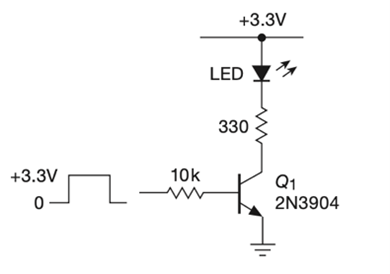
\includegraphics[width=0.25\textwidth]{LED.png}
    \caption{LED Circuit from the Art of Electronics}
    \label{fig:LED}
\end{figure}

\subsubsection{VESCs and Servos}
The \gls{vesc}s and servos required a similar output signal from the microcontroller, they both require a signal with a frequency of 50hz and a duty cycle between $ 1000\mu s $ and $2000\mu s $ \cite{pinckney2006pulse}. Using a PWM signal from the mbed board with a variable frequency controller, the Servo/ESC libraries written by the team worked effectively. This was deemed as the best solution for controlling the servos and ESCs for this project.

\subsubsection{Relays}

Since the relays already contained all the necessary circuitry, they only required a pin to be connected. The relays worked as expected for turning on and off the power to the main craft and thusly, the team agreed these were the best solution.

\subsubsection{Solenoids}\label{sec:sols}

Given the high-power drawing nature of solenoids, a specialist circuit was required for operation. It was decided that a Darlington pair was the most appropriate because they provide high current gain and can handle high currents and voltages with low power dissipation Additionally, Darlington pairs provide a high degree of isolation between the input and output circuits, which is important for protecting the control circuitry from voltage spikes and other transients that can be generated when switching inductive loads like solenoids.

\begin{figure}[h]
    \centering
    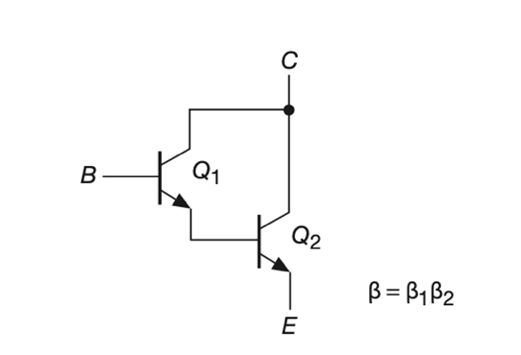
\includegraphics[width=0.25\textwidth]{dpair.png}
    \caption{Darlington Pair Circuit from the Art of Electronics}
    \label{fig:dpair}
\end{figure}

For the circuit a TIP120 (a Darlington pair in a single TO-220 package) was used, along with a flyback diode to protect against current spikes from the discharging inductive load of the solenoid~\cite{artofe_inductive_load,artofe_loads_and_doides}. A 47K resistor was used to act as a pulldown resistor and a 2K2 resistor to limit current draw by the transistor.

\subsubsection{Power Rectification}

Three-terminal fixed regulators were used for this project as they are deemed to be good enough for the job whilst being inexpensive to use~\cite{artofe_three_term_regs}. Three variations of an SOT-223 chips were used in a 3.3V, 5V, and 12V configurations. These were coupled with 100uF capacitors at their outputs to produce a smooth output voltage.
After testing, it was discovered that these SOT-223 chips were not adequate for power regulation in these circuits. Given that the power dissipated across these \gls{ic}s is equal to $P_{loss} = P_{in}-P_{out}=V_{in}*I_{In}-V_{out}*I_{out}$. With an input voltage of 16V and a power draw of 500mA and a voltage output of 5V, the power loss across these components was approximately 5.5W which over a small component was insufficient. This caused the regulators to overheat and cause failure of the components. Because of this, we upgraded these regulators to TO-220 with a large heat sink to dissipate the power. In the future a buck converter would be used to reduce the power loss due to the regulators.

\subsubsection{Switch and Button Input Debouncing}
To save overhead for the microcontrollers as well as reduce noise in the circuits, hardware switch debouncing was used on all the switches and buttons. This consisted of two main elements, a low pass filter tuned to 38Hz and a Schmitt trigger. The low pass filter was a basic RC filter that used 47Kohm resistors and a 100nF capacitors to create a 38Hz cut-off frequency~\cite{artofe_RC_circuit}. The Schmitt trigger was used on the output of the RC filter. A Schmitt trigger is a comparator (see §\ref{sec:comparator}) with hysteresis which operates on a threshold set to flip the output of the Schmitt trigger~\cite{parr1981schmitt}. The combination of the RC filter and Schmitt trigger gave a debounced signal from the buttons and switches to the microcontroller. This allowed for reduced overhead for the microcontroller as software debouncing of switches, which is relatively slow, was not needed~\cite{eejournal-switchdebounce}. After extensive testing, it was decided that this was the best method to debounce the switches on the circuits, the components were inexpensive and it stopped the microcontroller having to use delays to debounce the switches, ultimately slowing it down.

\subsubsection{Battery Level Monitors and Connection Test}\label{sec:comparator}
Both the battery-level monitors and connection test lines used comparators to provide their correct operations. A comparator is a close relative to operational amplifiers that have a high DC gain used to compare the magnitude of its two inputs. Comparators often switch within 100ns so can be considered almost instantaneous~\cite{parr1981}.

\subsubsection{Potentiometers}
Potentiometers were used for joysticks, threshold setting, and for fine-tuning of motor speeds. They were an important for of the control systems on board as they were used as the primary drive interfaces for the controller. Although relatively expensive, they were cheaper that using hall effect sensor alternatives for the joystick, which for a short-term prototype project were a good option. The threshold setting and tuning potentiometers were small surface mount devices which allowed the values to be changes and then set. This allowed for initial tuning of the values then they could be left, and the values would not change once this had been done.

\subsection{Controller Circuit}

The second circuit, the controller circuit, was responsible for reading the joystick positions, button presses, and switch polarity to enable the user to control the craft. It also provided audio and sensory feedback by utilising a buzzer and vibration motor. Furthermore, the circuit contained an LED collision sensor output array that provided collision detection and warning capabilities. Craft specific data such as steering mode and current speed of the motors is displayed using the onboard LCD. Most of the assemblies used in the schematic were identical to the ones used for the main board controller. The two novel components to the controller were the vibration motor and the buzzer. These have been outlined below.

\subsubsection{Piezoelectric Buzzer Circuit}
For the piezoelectric buzzer, comparators were used similarly to the LED switching in §\ref{sec:LEDS}. The biggest difference was that the piezoelectric buzzer required a 10kOhm resistor in parallel to allow the transducer to discharge whilst the transistor is off~\cite{ieee1666707}.

\subsubsection{Vibration Motors}
The vibration motor utilised the same circuit as the solenoids in §\ref{sec:sols}, given that the vibration is also a large inductive load. The same circuit was used again as it was serving the same purposed.  As well as working well for the solenoids, this circuit worked well for the vibration motor as operated as expected.

\subsection{PCB Design}

Once the circuit schematics were completed, PCBs were developed. These were important to create for the project because they have increased reliability and scalability over using other techniques such as breadboards or Veroboard. PCBs have more secure connections than breadboards ensuring better continuity between components whilst allowing a higher density of circuits per-unit-area due to the use of SMD components that would otherwise not be useable. For most of the PCB components SMD was used because they are significantly smaller than through hole components, they have enhanced electrical performance, and are most cost-effective than their through-hole counterparts. The enhanced electric performance is due to the shorter leads on the components which reduces parasitic capacitances and inductances within the circuit~\cite{springer-chapter-pcb}.  SMD also have a smaller footprint than through-hole components so the individual circuits can be placed closer to each other without causing interference. If THT was used exclusively for this project, the circuits would have had to be significantly larger to accommodate the additional size of the components.
Although more complex to solder, the team are happy with their decision to use primary SMD components on the board for the reasons stated above and if given the opportunity to redo the PCBs would do it in the same way again.

\subsection{Chassis and Kerb Climbing Design}

During the development of a robotic platform, optimal function and compatibility are important to consider with specific constraints. This section focuses on the design considerations for the chassis of the HEVCS, emphasising its dimensions, structural composition, and mechanical features.
The requirements set out in §\ref{sec:req}, prescribe limitations that the overall dimensions of the robot has to adhere to: a maximum height of 155mm; a maximum length of 2100mm; and a maximum width of 800mm. These dimensions were carefully considered such that the robot can fit under neither over 50\% of electric vehicles, through doorways in a domestic setting, and be able to fit into the lift in the development building. These were important considerations to ensure that the craft can be navigated around the final users’ home without significant modification. Therefore, the size restrictions as essential for guiding the design process of the chassis.

The chassis of the robot is constructed primarily of aluminium extrusion. For this application we considered other materials but ultimately decided that aluminium extrusion would be the best solution. Aluminium extrusion as the primary construction of the platform’s chassis offers numerus advantages. It is lightweight whilst also providing high strength resulting in a high strength-to-weight ratio that enhances mobility and energy efficiency whilst allowing for structural integrity.  The inherent rigidity of the material provides structural stability, allowing the chassis to withstand challenging operating environments. The channels of the aluminium extrusion allow for design flexibility allowing for the creation of complex structures to be iteratively developed whilst facilitating customisation and optimisation of the HEVCS platform.  The ease of fabrication, corrosion resistance and recyclability of the aluminium allow for a cost-effective, durable, and environmentally sustainable platform to be developed. Overall, these features make aluminium extrusion a desirable choice for constructing the chassis of the robot. It was these features that were discuss when deciding on using aluminium extrusion for the chassis. The selected extrusion of this project was 60mm in height and 30mm in width. This profile of extrusion was chosen because it offers a higher structural stability and load-bearing capabilities that the smaller profile of 2020 or even 2040 aluminium extrusion.

Given the intended functionality of the robot, the platform needed to be low-profile to fit under cars. But it also needed to be able to traverse kerbs of up to 150mm. As a result of this, the chassis incorporates articulated arms. These arms are multifunctional, they allow the HEVCS to climb kerbs, but they also hold the electronics to control the platform. These arms provide flexibility for the HEVCS to be able to ascend and descend kerbs without compromising on stability or structural stability. In addition to this, the arms of the robot are designed to facilitate the lifting of the robot’s frame to prevent it from being dragged along the floor whilst it is being moved. The arms of the robot are articulated using Super500 servo motors, known for their high torque and precise control capabilities. The Super500 motors have a torque of 500kg/cm (at 24V) and can facilitate precise accurate positioning of the arms of the platform.

One of the key design decisions of the HEVCS chassis was to make the design as user-repairable as possible. Given the nature of this build, it is important that the design is easy to take apart to facilitate for future developments and in the case of any damage occurring to the mechanism. Recognising the potential for mechanical failures or component damage, a user-friendly approach was taken ensure swift and hassle-free maintenance. By employing modular construction for parts such as the motor assemblies and using readily available fasteners and fixings, the chassis is able to be efficiently disassembled allowing for replacement or alternative parts to be easily installed and setup on the chassis.

The team are confident that the finalised design for the chassis for the HEVCS. The design has managed to fulfil all the criteria set out in the requirements section and has exceeded expectation in other ways. The final chassis height was only 110mm in high, allowing it to traverse under all bar one type of EV registered in the UK. The chassis can traverse kerbs and lift itself up and down as expected and the frame is solid being made from aluminium extrusion. The chassis design aligns well with the team's visions and objectives, which has ensured a functional and well-designed chassis for the HEVCS.

\subsection{Motor Assembly Design}

When designing the motor assemblies, there were a few important design considerations that needed to be accounted for. The motor mounts are a crucial component responsible for housing the drive motors, the belt drive, and mecanum wheels, whilst maintaining optimal performance and usability. To meet these requirements, they had to adhere to structural considerations and specific dimensions.
The motor mounts had a maximum height of 60mm to fit within the width of extrusion frame being used on the robot. This limitation was crucial for maintaining the overall compact nature of the robot and allowing it to still fit underneath the specified electric vehicles. As well as the maximum heigh of the motor mounts, they needed to be open at the wheel end of the assembly, this was to stop the wheels rubbing on the frame but also to allow the arms to move within their specified range of motion effectively.
Considering the high torque and power output from the drive motors, it is important to ensure that the drive system was mounted in a manner that prevented bending and flexing of the mount, even under large loads. This necessitates a robust mounting system to maintain the systems integrity and stability during operation. The motor mount is secured to the extrusion using the inside plate using six 6mm bolts. This provided a reliable mounting platform within the chassis of the main platform.
The mecanum wheels are driven from the motor using a belt drive system. Despite considering many types of drive options such as, gear drive, chain drive, and direct drive, the team ultimately decided to use belt drives. The reason being that gear drives have a high capability and capacity for torque transmission and can present a compact design. However, its limited shock absorption makes it less suitable for application in a platform that will be required to climb up and down kerbs and uneven terrains, where reducing vibrations is crucial. Chain drives offer a high load capacity with a robust design but require frequent lubrication when used for high torque applications. Chain drives also have potential for increased complexity which further influenced our decision as we aimed for a simpler solution. Although used for the initial prototype design, the team decided against the use of direct drive for the final HEVCS platform. Whilst be useful for control and efficient power transfer, the motors would not have been able to operate within their optimal range to allow the best torque and efficiency. Ultimately, belt drives were used due to their significant advantages for our specific application. Belt drives offered a smooth and quiet operation, tolerance for misalignment, shock absorption and inherent overload protection. If the torque on the belt is too high, the belt will slip preventing damage being cause to either the motor or the wheels. Belt drives were also the most cost-effective solution when compared to belt and chain drive systems. The belt drive system featured a 2:1 gear reduction to allow for optimal power and torque transmission. Belt tensioners, made from a free running pulley, were used to help reduce slippage from the belt drive. This pulley allowed for adjustment in the belt to allow for adjustment of the belt as it stretches throughout use.
The finalised design for the motor mount was exactly 60mm in height (not including the motors and wheels), and mounts onto the inside of the chassis extrusion. The axel for the mecanum wheel is supported at three points throughout the frame using three pillow-block bearings. This was done to provide stability for the axel and to reduce the friction on rotation.

% NEED TO INCLUDE REDNER IF ROOM PREMITS

Motor assembly modularity was one of the most important features of the motor mounts throughout the design and construction phases of this project. The motors mounts were designed to be modular to allow for streamlined integration, scalability, and ease-of-repair. By designing the motor modules in this way, an increase in the speed of integration was made, and it resulted in a positive environmental impact. The environmental benefits of modular designs include resource efficiency, extended product lifespan and sustainable upgrading of assemblies and modules.
Overall, the team were very happy with the motor mount design. The motor was suitably reinforced, and the wheel was suitably supported. The belt drive was smooth, reliable, and quiet during operation and allowed for slight misalignments in the mechanism without causing slippage or the belt to fall off the pulleys. The mounts were strong and did not flex under the weight of the craft and the team are confident that it would have been able to support the full weight of the platform with ease. The only issue with the motor mounts was the gear reduction used. Upon reflection, a 2:1 reduction was insufficient for the motor to operate effectively. If re-designed, a 4:1 or higher reduction would have been used to allow the motor to spin faster and be able to more comfortably to operate at its peak-efficiency whilst maintaining a controlled speed at the wheels.

\subsection{LiDAR Placement and Mounting Design}
To provide 300° coverage, and to minimise blind spots in vision-critical regions, the LiDARs were mounted in dual-mounts. Vision-critical regions are areas that have the highest probability of an obstacle appearing in. The main regions in figure \ref{fig:lidar_plac} are directly in front of the front and back faces.

% \begin{figure}[H]
%         \centering
%         \begin{subfigure}{width=0.5\textwidth}
%             \centering
%             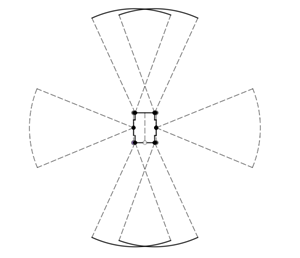
\includegraphics[width=50mm]{lidar_placement_old.png}
%             \caption{Original LiDAR Placement}
%             \label{fig:lidar_plac_old}
%         \end{subfigure}%
%         \begin{subfigure}{width=0.5\textwidth}
%             \centering
%             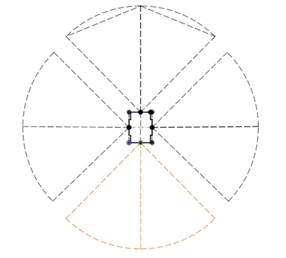
\includegraphics[width=50mm]{lidar_placement_new.png}
%             \caption{Revised LiDAR Placement}
%             \label{fig:lidar_plac_new}
%         \end{subfigure}
%         \caption{Comparison of LiDAR Placements}
%         \label{fig:lidar_plac}
%     \end{figure}

The original design in figure \ref{fig:lidar_plac_old} utilised six LiDARs placed around the chassis, one on each corner facing forwards or backwards, and one on each side, perpendicular to the others. This arrangement, while allowing for cross-referencing between adjacent LiDARs, had large blind spots on the corners, and a 1030mm blind spot in the centre of the front and back. This large a blind-spot in a vision-critical region was considered unacceptable, and so the design was changed.

The adjacent figure \ref{fig:lidar_plac_new} shows an alternative mounting schema using an additional two LiDARs, bringing the total to eight. This arrangement, made up of centre-mounting the LiDARs at an angle that minimises overlap while doubling the field of view to 89°. This design limits the blind spots to a 755mm strip extending from each corner of the design. Whilst blind spots still exist, they are no longer in critical-vision regions, and so are less of a concern. Caution should still be taken by users, however, as obstacles within these diagonal regions may be an issue when using the strafe mode.

\begin{figure}[h]
    \centering
    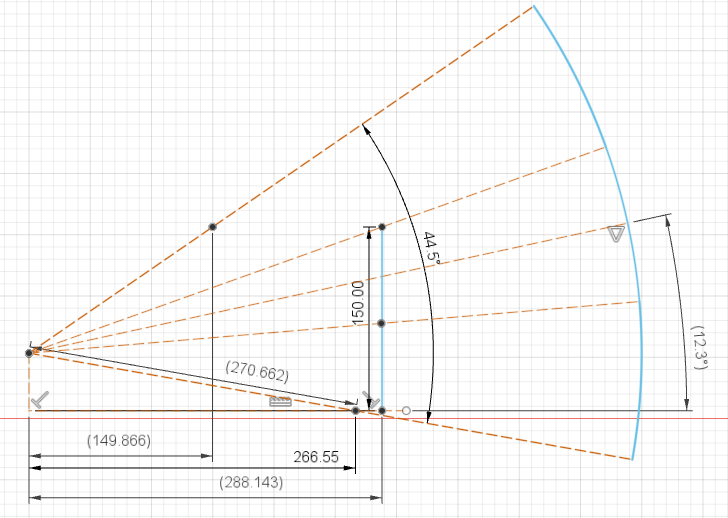
\includegraphics[width=0.25\textwidth]{LiDAR_PLACEMENT_GRAPH.png}
    \caption{Diagram of LiDAR angular placement}
    \label{fig:lidar_plac_graph}
\end{figure}

With the 47mm mount height, the lower half of the LiDAR beams would be pointed at the ground for most of the operation, effectively halving the useful number of samples the sensors would take. To prevent this, the LiDAR mounts were angled upwards by 12.3°,  improving the minimum distance of the obstacle height calculations to 150mm, and the distance at which the lowest row of sensors begins the reading the ground to 266mm.
\subsection{LiDAR Mount Design}

% \begin{figure}[h]
%     \centering
%     
\includegraphics[width=0.25\textwidth]{l_mount_old.png}
%     \caption{Original mount design}
%     \label{fig:l_mount_old}
% \end{figure}

Following the initial mounting schema, the Lidar mounts were initially to screw into the ends of the chassis extrusion lengths, pointing the LiDARs forwards. Figure \ref{fig:l_mount_old} shows a render of one of the corner LiDAR mounts. The two screw holes in the recess match with the screw holes on the Pimoroni breakout board. The recess is designed to prevent the breakout board from extruding beyond the surface, reducing the chance for sensor damage should a collision occur. A rectangular cut out provides a routing channel for the LiDAR connectors.

TWO LIDAR MOUNT RENDERS HERE FiX REF below

Figures  and  show the redesigned centre and side Dual LiDAR mounts. Using the aforementioned calculations, the LiDARs are offset horizontally, maximising horizontal field of view. The centre mounts include screw holes to allow mounting to the top plates of the armatures, while the side mounts include side flanges to allow them to be secured to the side extrusion using T-nuts. Corners are chamfered to provide additional strength, reducing stress concentration at corners\cite{BELINGARDI2002273}.
For the prototype, each mount was printed using PLA, chosen out of the available plastics for 3D printing for a combination of its relative strength, ease of printing, and low cost. For a production run of the product, a more permanent solution can be found, but for an initial prototype the inherent advantages of 3D printing for rapid prototyping made PLA a perfect choice.

\begin{table}
    \begin{tabular}
    {|p{2.1cm}|p{1.8cm}|p{2.1cm}|p{2.1cm}|p{3.1cm}|p{3.2cm}|}
    \hline
        Material & Cost & Strength & Rigidity & Ease of Printing & Tolerance \\ \hline
        PLA & LOW & MID & MID & EASY & Approx 0.4mm\\ \hline
        TPU & MID & LOW & LOW & HARD & 0.4mm\\\hline
        RESIN & HIGH & HIGH & HIGH & EASY & $>$0.1mm\\\hline
    \end{tabular}\\
    \caption{3D printing material comparison}
    \end{table}
\subsection{Breakaway Connector}

A breakaway connector was design to add an additional safety measure when operating the craft. The breakaway connector is positioned along the cable connecting the controller to the craft, providing a reliable connection while allowing for detachment should the circumstance occur. Magnets are incorporated at the centre of each connector so that if the craft begins to move too far away from the user, the connection will be lost, and the craft will come to an immediate stop. 

The breakaway connector comprises of two main components: the PCB and the casing. On the male face of the PCB, a set 10 pogo pins organised in a circular pattern which will come in contact with corresponding SMD pads on the female connector PCB. The PCBs have a radius of 20mm and feature a central hole of radius 7mm to allow space for the magnet. Since KiCad does not have a feature to make a circular pattern, a MATLAB script was written that provides coordinates around circumference of a circle.

For each end of the connector a case was fabricated using a 3D printer. The cases protect the PCBs from external factor that might affect the functionality and provide housing for the magnets. A triangular notch was incorporated into the design to stop an improper configuration during connection. This notch prevents incorrect alignment and ensures the power lines are correctly oriented, removing risk of damage to other connections.

The design of the breakaway connector considers both safety and practicality and a render can be seen in \ref{connectorRender}. The neodymium magnets provide a 3.6kg pulling force enabling a secure detachable connection, while ensuring that the draft can be safely operated within a certain proximity to the user. 
The team were happy with the performance of the breakaway connector. It provides a secure connection which can be broken should the circumstance occur. The casing protects the PCBs and holds the wire casing in place. While the breakaway connector worked well, further improvements could be made. The 3D printed case has some imperfections which can make it difficult to align the connectors correctly. Also, the rim around the pogo pins should be longer so that it can protect the ends of them from damage.

\begin{figure}[h]
    \centering
    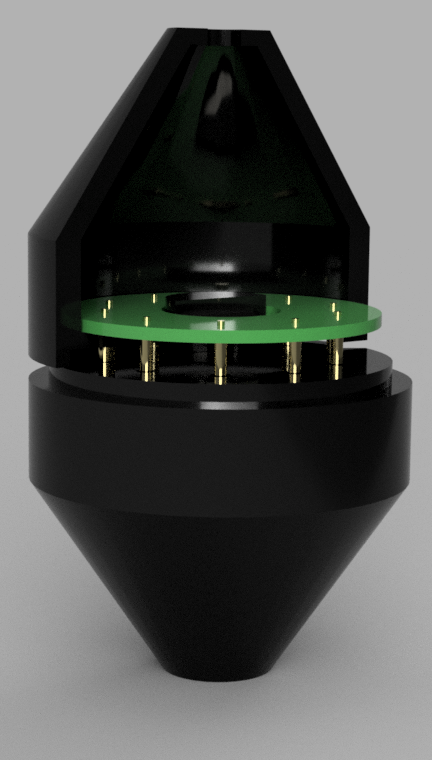
\includegraphics[width=0.25\textwidth]{ConnectorRender.png}
    \caption{Render of the Breakaway Connector}
    \label{fig:connectorRender}
\end{figure}


\newpage
\section{Software Design} \label{sec:softwareDesign}

\newpage
\section{Testing}

\subsection{Software Testing}
When testing the software for the project, a set of testing requirements and a testing schema was used. The first step of software testing was a requirement analysis to understand the functional specifications of the system. The next step taken was test planning and test case design. These steps were used to define the objectives of testing and to determine the testing techniques to be utilised. Testing documentation was then needed to be developed to track all the tests that have been undertaken and define the inputs, outputs, and expected results from all the testing schemas. After the tests have been devised, the test environments are setup, and the tests are executed. Once this has happened, the results are analysed and any issues with the tests are handled using the appropriate manner.  Regression testing was then done to check that the newly added features did not negatively affect the old tests that were run. Validation and verification are then completed to check that the software meets the expected outputs under various operating conditions. After this the documentation is updated and a final testing report was created. 

The STM32 development ecosystem provided comprehensive support for software testing. The STM32Cube software development platform includes tools and utilities for debugging, profiling, and testing, ensuring efficient detection and resolution of software issues. Additionally, third-party testing frameworks and tools, such as unit testing frameworks and code coverage analysis tools, are readily available and compatible with both mbed and STM32 platforms. These testing resources enabled the team to conduct rigorous testing and verification of their software, enhancing overall system quality. Furthermore, the STM32 boards are built on open standards and offer open-source software development environments.  

Upon reflection, the team would like to use STM32Cube more in this project, and in the future, as it provides an open and flexible platform for software development, including libraries, middleware, and development tools. This openness enabled the team to access and modify the underlying software components, facilitating customisation, bug fixing, and optimization. Openness also encourages community contributions, resulting in continuous improvements and a collaborative testing environment, values of which result in the team’s increased passion for embedded software.
The team also identified a possibility for more software-integrated error handling, such as try-throw-catch blocks in C++ and try-except-else-finally blocks in Python, both of which allow custom exceptions to be created and handled in defined ways.


\subsubsection{Main Board Software Testing}
The main board software was tested using the framework outlined in §(INSERT SECTION MARKER). The software for the main board was tested using bottom-up integration, an approach based on testing individual components (or units) first and gradually integrating them into larger subsystems. It is a method of integration testing that starts from the lowest level of the architecture and moves up until the system is comprehensively tested. 

Testing began by toggling the LEDs on the board, then moving onto generating VESC outputs using PPM control. Once this was done, the two units were added together and then tested as a cohesive unit. This showed that the functionality of both blocks of code did not affect the operation of each other. This is was done for all the other functionality outlined in \ref{sec:softwareDesign}. Once all the functionality was tested, the board was then installed into the main craft and integration testing was done with the hardware. This was done to ensure that there were no conflicts from the code that negatively affected the software. 

During operation the software on the main board worked mostly as expected most of the parts of the software work coherently and correctly. There were a few conflicts on Interrupt Lines and Busses, which required the changing of pins on the PCBs. Whilst this was time consuming to rectify it ultimately did not affect the overall functionality of the main board which continued to work as expected. 

\subsubsection{Driving, Steering and Motor Control Testing}
The motor control was obtained using PPM signals. PPM is similar to PWM signals that are used in standard RC remote control \cite{ppm}. The signals used a varying signal time between 0.5ms and 1.5ms on top of a 50Hz PWM output. This signal was then passed into the VESCs that were used to drive the motors. 

The driving algorithm for the mecanum wheels is a complex set of equations that utilise trigonometry to calculate the correct speed and direction for the motors to rotate to travel in a specified direction. As a result of this, the equations and output from the algorithm required significant testing. The algorithms were initially tested using a python script utilising the build in ‘pytest’ library. This was used to evaluate test cases for the motor algorithms including the joystick at 0,0; 10,0; -10,0; etc. These tests were successful, indicating the algorithm was ready to deploy in C++ in an embedded context. 

Once the driving algorithm was tested, it the steering algorithm could then be implemented. The steering algorithm was more simplistic than the driving algorithm. It only required to speed up or slow down the motors at a linear rate depending on direction the user wants to turn in and the speed they wish to turn in. 

The Steering, Driving, and Motor Control was all successful and the team are confident that the best methods for controlling the motors was chosen. The VESCs were the best choice for this project as they provided a simplistic user interface which did not require extensive to control or external hall effect sensors to operate. If a higher precision control system was required, O-Drives would have been a better choice for a control system. 

\subsection{Hardware Testing}

\subsubsection{PCB Testing}

The process of testing PCBs involves several steps to ensure proper functionality and reliability. The team started by visually inspecting the PCBs to check for any visible defects such as solder bridges, misplaced components, or damaged traces. This visual inspection may help identify any defects on the board that may cause an issue to the board’s performance. On initial visual inspection of the board when they had arrived, the controller board was missing the top layer silkscreen, which whilst not an issue with functionality, did cause disruptions to the soldering process. 

Once visually inspected, the team performed continuity testing on the boards using a multimeter. By probing different points on the boards, the team ensured that the electrical connections on the board were intact and that there were no open circuits.  Upon testing on the PCBs there were a few places which required resoldering, which if not been checked would have caused issues with debugging later in the process. 

The next step the team performed was basic power-on testing. Once the continuity of the PCB was performed, the PCB was powered using a lab power supply with a current limit. The board was then probed again using a multimeter to test that the correct voltages and currents are present within the circuit. This stage helps identify any power issues, abnormal heating, or voltage irregularities. 

The final two stages of the PCB testing that the team undertook were functional and performance testing. Functional testing was used to validate the operation of the PCB by simulating real-world input and output conditions. The team used specific signals and inputs to the boards to evaluate the outputs that were received. This was done in using the onboard microcontrollers and some C++ testing firmware. This step verifies that the PCB performs as intended. Performance testing was then done which is very similar to functional testing but loads the PCB more to test it can work under a variety of challenging conditions. 

Once the testing was completed, the team was satisfied that the PCBs worked as expected. 


\subsubsection{Motor Mount Testing}

Several types of testing were implemented at each stage to evaluate the performance and reliability of the motor mounts and associated components.
During the initial design stage, a non-load bearing test rig was utilised to assess the functionality of the motors and their integration with the VESCs, using the VESC Tool software. Functional tests confirmed that the motors could be successfully activated and controlled using the software. However, when a wheel was mounted to the motors, the mounts experienced vibrations causing them to shear along the layer lines.

The motor mount design was revised to address the stability and structural concerns. The new design supported the wheel on both sides and were robust enough to support a basic square aluminium chassis. These mounts allowed for the testing of the drive system as outline in section ??. 
Further tests were conducted on new motor mounts which included a belt drive system. Initially, the distance between the pulleys was too short for the belt, so the distance was revise ensuring optimal belt engagement and preventing slippage. To further improve the reliability of the belt drive, a tensioning pulley was implemented, through the addition of a slot on the plates. Overall, the motor design demonstrated smooth and quiet operation during testing.

Stress tests were conducted throughout the testing process confirmed the strength and durability of the motor mounts. They exhibited resistance to breakage, deformation, and failure when subjected to controlled forces and loads. This indicated their ability to withstand the operational test demands placed upon them.

Subjective testing provided insights into the performance of the motor mounts. Observations revealed no significant vibrations or abnormal noise during operation, indicating satisfactory stability, smoothness, and overall quality. 

Based on the comprehensive testing results obtained at each stage of development, the motor mounts were integrated into the HEVCS. The results validated their functionality, strength, and compatibility, ensuring their reliable performances within the system.

\subsubsection{Design}

Once the chassis was assembled, a number of tests were conducted to evaluate its performance and capabilities. The testing focused on key aspects such as the articulation of the arms, the payload weight limits, the lifting capacity of the chassis, and the platform’s ability to navigate obstacles.

The assembled chassis underwent an assessment of its articulation capabilities. This involved examining the movement and flexibility of the arms. The objective was to ensure smooth operation and unrestricted articulation, enabling the platform to navigate various terrains. Visual inspection along with manual manipulation of the arms confirmed that the arms have the full range of motion they require.

Once range of motion was assessed, the maximum weight that the chassis can handle, within the limit set out by the legislation, was assessed. Incremental weights were added in 10kg intervals up to 80kgs, were used to measure the chassis’ payload capacity. The test showed that the platform is capable of being driven while carrying 80kg.

Nex the lifting capacity of the chassis was evaluated. Initial tests revealed that the super 500 servos, powered by a 16V supply, struggled to lift the chassis, which weighed 31kg. However, when using a 24V power supply, the servos showed an improved performance, successfully lifting the chassis without encountering any issues. This test revealed that the servos required a greater voltage supply than initially thought.

Additionally, a mock-up of a step with a height of 150mm was constructed to test the platform’s ability to fit underneath an electric vehicle and its ability to climb a kerb. Since the platform had a height of 110mm, it was successfully driven underneath the mock-up step. However, power issues prevented a comprehensive assessment of the platform’s kerb climbing capabilities, the results obtained from previous tests provided confidence in its ability to navigate such obstacles successfully.

Overall, the testing phase demonstrated the functionality and performances of the HEVCS. By examining each functionality of the arms, the testing process validated the system’s effectiveness and provided valuable insights for further refinement and optimisation.


\subsection{Inter-board Communications Testing}

A variety of communications protocols were used during the development of the project, each with different strengths and weaknesses leading to differing applicability. I2C was primarily used for short-range communication, intra-board where possible. A combination of SPI and UART was used to communicate over longer distances. The code in figure \ref{} shows a fragment of one half of the UART test code, complete with timing. On average, a UART transmission took $\approx$ 85 CPU ticks to complete, and data integrity was preserved throughout.

	Wherever data transfers occurred, data validation was used to ensure incorrect data was not taken into the system. In particular, as several communication busses had discreet contents – that is, the contents of each data packet could only be one of a few possible values -error checking was simple.  

Figure \ref{} shows one example of a try/except statement designed to catch invalid data. By attempting to read the second entry of the data list, the code checks to see if at least two values have been received. If not, the data is not processed, as continuing would lead to an out-of-index exception. 

\subsubsection{Binary Encoding Testing}
To test the threshold detection and binary encoding, random sets of variables were generated, and then fed into the comparison function. These variables are then displayed on the terminal. This testing method does require human comprehension of the output, however high confidence in the code can quickly be reached with only a subset of values tested. Edge and corner cases were specifically tested for compliance.

\subsection{LiDAR Accuracy Testing}
To test the accuracy of the LiDARs, they were placed in a vice, and pointed at a flat plywood sheet a fixed distance away. For the purposes of this test, the plywood sheet had an approximate 30\% reflectance value, and lighting conditions were ambient.

\begin{table}[]
    \begin{tabular}{|l|l|l|l|}
    \hline
    \textbf{Distance (mm)} & \textbf{Average Reading (mm)} & \textbf{Error} & \textbf{Error \%} \\ \hline
    \textbf{5}             & 4.02                          & -0.98          & -19.60\%          \\ \hline
    10                     & 10.5                          & 0.5            & 5.00\%            \\ \hline
    15                     & 16.43                         & 1.43           & 9.53\%            \\ \hline
    20                     & 19.74                         & -0.26          & -1.30\%           \\ \hline
    25                     & 26.22                         & 1.22           & 4.88\%            \\ \hline
    30                     & 27.4                          & -2.6           & -8.67\%           \\ \hline
    100                    & 107.01                        & 7.01           & 7.01\%            \\ \hline
    150                    & 159.8                         & 9.8            & 6.53\%            \\ \hline
    200                    & 184.66                        & -15.34         & -7.67\%           \\ \hline
    250                    & 233.58                        & -16.42         & -6.57\%           \\ \hline
    300                    & 281.06                        & -18.94         & -6.31\%           \\ \hline
    500                    & 532.89                        & 32.89          & 6.58\%            \\ \hline
    750                    & 794.32                        & 44.32          & 5.91\%            \\ \hline
    1000                   & 1096.73                       & 96.73          & 9.67\%            \\ \hline
    \end{tabular}
    \caption{LiDAR measurement testing results}
    \label{tab:lidar_res}
    \end{table}

Table \ref{tab:lidar_res} shows a subset of testing result. The sensor performed better than expected, the error remaining within the bounds specified within the sensor’s datasheet. It should be noted, however, that the two targets the datasheet’s testing used had a reflectance of 17\% and 88\% respectively, and ambient light was fixed at 5kilolux, so these results are not directly comparable.




\newpage
\section{Evaluation}

\subsection{Leadership Methodology}
The team adopted a democratic approach, and although various ideas to solve problems were explored, there were no disagreements during development. Individual team members worked on tasks they had relevant experience in, enabling the sharing of knowledge while facilitating fast development. However, to honour the NDA, the team had to work in a separate room to the rest of the cohort. This was beneficial at times but resulted in less outside perspectives from university colleagues. This was recognised by the team as they chose to remain objectively critical and seek feedback from those deemed appropriate. The team acknowledge that the way in which they operated as a team was effective, but upon reflection wish that more academic feedback was sought throughout.

\subsection{Project Progression}
The project’s development reflected the GANTT chart up until the middle of March. At this point, the team changed the design to make it more modular, requiring further testing and a redesign of the chassis, motor, and servo mounts. The team do not regret this change to the design as it greatly increased the platform’s performance and functionality. This did, however, have an impact on the aesthetics of the platform as the outer casing manufacturing was delayed.  The team discussed this and determined that functionality was more important, and that the overall structural integrity did not rely on the casing. Furthermore, the way in which the project progressed through the defined stages of development was assessed through \gls{kpi}s and tests indicative of successful completion of a milestone. The team felt that combining this with the agile methodology meant that no developmental steps were missed, as everything was regularly reviewed directly from the critical development pathway.

\subsection{Corporate Sponsorships}

\subsubsection{Sirmon Industries}
James and Heather Sirmon attended on-site meetings every week. Heather was critical of the project, pushing the team to consider the wider application of the \gls{hevcs} as a real-world product. She questioned our decisions, while James queried our justifications as he completed the patent application. Additionally, their regular reviews enabled the team to discuss the progress and decisions in detail, meaning that Sirmon Industries Limited were satisfied as a customer. The team feel that they completed the project in a professional manner and are glad to continue work with both Sirmon and the company that further develop the \gls{hevcs}.

\subsubsection{European Social Fund}
Jo Byrne was available to discuss the commercial viability of the \gls{hevcs} during its development. The team often reflected on the capabilities of the project in relation to legislation, as well as defining the novel aspects that Sirmon required for the patent application. The insight provided by the \gls{esf} was vital for understanding the customer usability of such a device, and how the outside opinion of those who do not have the technological understanding can provide interesting perspectives from a customer’s point of view.

Two reports were produced for the ESF, each covering various aspects of the project requirements and the methodology. This meant that at the start of the project each team member did a skill set review that was then used to determine who would develop what specific elements of the \gls{hevcs}. Halfway through the project, the final ESF report was due. It detailed the roles that the members of the team grew into, the milestones that had been completed, test methods used, and the business recommendations for Sirmon Industries. This helped the team to gain an insight into how the project could be developed further, while defining the scope for the \gls{hevcs}’s development as a university project.

\subsection{Budget Management}

The university provided £1,200 in budget, and Sirmon Industries allotted £2,000. The team decided to create a bill of materials for the entire project to coordinate arrival times, costs, and availability. As the university had an approved list of suppliers, the products that were not on this list were automatically sifted to the \gls{bom} to be discussed with Sirmon Industries. It is worth noting that the components purchased were still deemed appropriate for the project, and therefore approved by the university academics. The external supplier \gls{bom} also included products with a long lead time, that James Sirmon was able to source from his industry partners instead. These decisions were beneficial to the project’s initial development, and the team believe they made the correct choice by asking Sirmon to obtain such components during the Christmas break, a period in which the university could not place or receive orders.

Portions of the university budget were allocated for electronic components, manufacturing costs, and materials. This included the PCB component orders from approved suppliers that the university had existing free, fast shipping subscriptions with. The team felt that this decision was correct, enabling fast acquisition of vital components for chassis, motor, and hardware assembly too.

A complete breakdown of the costings can be found in the appendix. This includes a breakdown of how £1,163 of the university budget was spent, and how Sirmon spent £1,862.76. The remaining balance was £174.25. The team acknowledge that a large proportion of the costs, equating to 500 came from purchasing \gls{vesc}s. Designing a speed controller for this project would have been time-consuming, whereas a fast, reliable, and sufficiently documented solution was required. Thusly, the project benefited from using the \gls{vesc}s, their convenience and their positive impact on the initial platform control testing.

In conclusion, the overall cost of this project far exceeded the budget provided by the university, and so the team would like to acknowledge the contributions from Sirmon Industries and extend their gratitude. It is through their generosity that the project was able to progress, possess high quality products, and operate effectively.

\subsection{Customer Usability}

The \gls{hevcs} is reliably controlled by the user, using methods that enhance its dependability. The purpose behind the prototype is to prove its potential as an alternative method to EV charging, using methods and approaches that the user can rely on and independently control. Using the results of the \gls{mece} analysis that define \gls{ev} owner’s needs to a dependable solution to charging at the convenience, the \gls{hevcs} has proven itself as a viable alternative. Moreover, its creation presents a viable alternative to getting power to the vehicles, provided they are within a certain proximity of the home, that is not limited by obstacles such as kerbs.

This paper has detailed how the cost of charging is decreased using off-peak domestic tariffs, enabling the user to effectively control the price they pay to charge their EV using electricity schemes. Giving the user authority over when, how, and how much they charge their vehicle increased the accessibility of owning an EV.

\subsection{Ethics}

The ethical conduct principles defined in the PEP have been applied throughout the development of the \gls{hevcs}. A deeper understanding of the operational safety of the platform has been acquired through testing, and several efforts have been made to limit the risk of injury to both users and the public through the deployment of several safety features discussed in the design section. Namely, the magnetic breakaway cable and the object avoidance system. The team have made an effort to create safety systems that enhance human capabilities without revoking their control. For example, users can drive the platform towards a wall, and the object avoidance system will prevent them from making contact with said wall, but it does not take away their ability to continue to operate the platform in another direction that does not cause harm. Furthermore, the platform is not autonomous, as to abide by the relevant legislation, and so the public are ensured that humans retain all control of such a device.

The research conducted throughout this project has included the use of and reference to data from national surveys, from which the participants have agreed to the distribution of their information. The team have not gathered or collected information themselves nor obtained any data through the university.

\subsection{Environmental Impact}

The environmental impact of the components and products used to build the \gls{hevcs} have been discussed in their relevant sections. Furthermore, the future improvements include discussion of alternative methods of acquiring power through sustainable, green energy sources. The team would like to reiterate the importance of recycling \gls{ev} batteries, building on the explanation on the impact on the environment discussed in the \gls{pep}.

Multiple characteristics of \gls{bldc}s result in a reduced negative impact on the environment. They require less energy to operate than DC or AC induction motors. They are more efficient in terms of energy loss and durability, meaning they need replacing less often and therefore produce less waste. As they do not have brushes, there is no carbon dust or other emissions produced during operation, including noise emission. However, the team acknowledge that the environmental impact is dependent on the motor’s application. This means that power consumption was limited through decisions within the software and the platform’s operation. This includes features such as regenerative breaking and speed limitations.

\subsection{Design}

The team is pleased with the overall design of the \gls{hevcs} prototype platform and its capabilities, as the maximum height of the platform exceeded the target of 150mm. With a final height of 110mm, the \gls{hevcs} is able to fit under all bar one of the types of registered electric vehicles in UK \cite{carsinit}. Due to the confidential requirements in place for the project, the design was not able to be tested outdoors. However, the team is confident that with suitable levels of testing and a small amount of modification the \gls{hevcs} would be fully operational outdoors, on both pavement and road surfaces.

During testing, the craft demonstrated stability and the ability to support a payload of up to 80kg before collapsing, aligning with the requirements of the project. As well as this, the craft fully abides by all relevant class 2 mobility scooter legislation, allowing it to be used on pavements.  Furthermore, preliminary testing strongly suggests that the platform has the potential to navigate and manoeuvre over kerbs, of up to 150mm, with further developments and refinements. This promising outcome bodes well for the future optimisation and further developments of the platforms design capabilities.

Overall, the team is satisfied with the design prototype. This stems from its successful and complete adherence to the requirements of stability, weight capacity, and also for its potential developments in kerb climbing ability.

\newpage
\section{Further Developments}

While the HEVCS in its current form, performs to a good standard, there are still some areas in which improvements can be made. These include power systems, reducing height, and integration of the payload.
Throughout the development process of the HEVCS, several challenges were encountered in relation to the power systems on the PCBs. A significant issue involved the voltage regulators, as they were unable to handle the step-down of current without being attached to a heatsink, in the form of aluminium extrusion. This limitation gave concern with the long-term reliability and thermal management of the power circuitry. As a result, further improvements of power circuitry need to be implemented.
Another complication arose during development during transmissions from the main board to the VESCs. This was due to the VESCs and main board not sharing a common ground, which was solved by grounding the entire chassis so that a ground plane had to be implemented. For future designs, a more robust and safer ground plane will need to be implemented.
In the existing design of the HEVCS, the arrangement of the motor leads going to the VESCs is contributing to the overall height of the system. To address this issue, a hole can be added to the piece of extrusion that is behind the motors. With this addition, the motors can be laid flat so that the cables can be coming out the back instead of the top. This will reduce the height by approximately 20mm.
Currently the super 500 servos are being powered by batteries that supply a voltage of 14.8V. While this voltage falls within the operational range of the servos, to get the maximum torque of 500kg.cm, they require 24V supply. By providing the servos with the maximum voltage, the system can ensure optimal performance and maximise the torque output required for its intended application.
Additionally, the batteries that are being used to power the motors do not have a large enough capacity to allow for enough runtime. To take this project further batteries with a greater capacity need to be found. For 30mins of runtime, the motors will need a battery with a capacity of 12 Ah. Alternatively, the motors can be powered from the payload compartment. While this would reduce the amount that the EV can be charged, it will reduce complexity when it comes to charging the system.
To fully test the capabilities of the systems, the payload compartment of the HEVCS needs to be loaded with retired EV batteries. Additionally, the necessary components and infrastructure must be incorporated to facilitate the charging of EVs using these batteries. This testing phase would allow for an evaluation of the entire systems performance, efficiency, and overall effectiveness in delivering the intended charging capabilities. Testing under realistic conditions, any potential issues or areas of improvements can be identified and addressed.
Sirmon Industries Limited are actively pursuing further development of the HEVCS by collaborating with a third party. Their aim is to transform the HEVCS into a commercially viable product that will be available for purchase by consumers. Recognising the potential of the system and its significance in addressing the growing demand for EV charging solutions, Sirmon Industries Limited has filed a patent application.


\newpage
\section{Conclusions}

\newpage
\bibliographystyle{IEEEtran}
\bibliography{ref.bib}

\newpage
\appendix

\section{Appendix A: Project Documentation}

\section{Testing}

\begin{figure}[h]
    \centering
    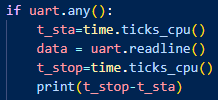
\includegraphics[width=0.25\textwidth]{uartTest.png}
    \caption{}
    \label{fig:uartTest}
\end{figure}

\begin{figure}[h]
    \centering
    
\includegraphics[width=0.25\textwidth]{uartTestData.png}
    \caption{}
    \label{fig:uartTestData}
\end{figure}

Project OneNote \cite{onenote}
Module OneDrive \cite{unidrive}
Private OneDrive \cite{privdrive}

Finalised BoM \cite{bom}
Risk Assessment and COSHH Forms \cite{RA}

GitHub Repository \cite{}

\end{document}